\documentclass[a4paper,12pt]{article}

\usepackage[T2A]{fontenc}			
\usepackage[utf8]{inputenc}			
\usepackage[english,russian]{babel}	

\usepackage[
bookmarks=true, colorlinks=true, unicode=true,
urlcolor=black,linkcolor=black, anchorcolor=black,
citecolor=black, menucolor=black, filecolor=black,
]{hyperref}

\usepackage{color}
\usepackage{caption}
\DeclareCaptionFont{white}{\color{black}}
\DeclareCaptionFormat{listing}{\colorbox{white}{\parbox{\textwidth}{#1#2#3}}}
\captionsetup[lstlisting]{format=listing,labelfont=white,textfont=white}

\usepackage{amsmath,amsfonts,amssymb,amsthm,mathtools} 
\usepackage{wasysym}

\usepackage{graphicx}
%\usepackage[cache=false]{minted}
\usepackage{cmap}
\usepackage{indentfirst}

\usepackage{listings} 
\usepackage{fancyvrb}

\usepackage{geometry}
\geometry{left=2cm}
\geometry{right=1.5cm}
\geometry{top=1cm}
\geometry{bottom=2cm}

\setlength{\parindent}{5ex}
\setlength{\parskip}{0.5em}

\usepackage{pgfplots}
\usetikzlibrary{datavisualization}
\usetikzlibrary{datavisualization.formats.functions}

\begin{document}
	\lstset{ %
		language=C,                 % выбор языка для подсветки (здесь это С)
		basicstyle=\small\sffamily, % размер и начертание шрифта для подсветки кода
		numbers=left,               % где поставить нумерацию строк (слева\справа)
		numberstyle=\tiny,           % размер шрифта для номеров строк
		stepnumber=1,                   % размер шага между двумя номерами строк
		numbersep=5pt,                % как далеко отстоят номера строк от подсвечиваемого кода
		backgroundcolor=\color{white}, % цвет фона подсветки - используем \usepackage{color}
		showspaces=false,            % показывать или нет пробелы специальными отступами
		showstringspaces=false,      % показывать или нет пробелы в строках
		showtabs=false,             % показывать или нет табуляцию в строках
		frame=single,              % рисовать рамку вокруг кода
		tabsize=2,                 % размер табуляции по умолчанию равен 2 пробелам
		captionpos=t,              % позиция заголовка вверху [t] или внизу [b] 
		breaklines=true,           % автоматически переносить строки (да\нет)
		breakatwhitespace=false, % переносить строки только если есть пробел
		escapeinside={\%*}{*)}   % если нужно добавить комментарии в коде
	}
	
	% Титульный лист
	\begin{figure}[h!]
		\begin{center}
			{
\includegraphics[scale = 0.4]{titul.jpg}}
			\label{titul}
		\end{center}
	\end{figure}
	
	\vspace*{15mm} 
	
	\huge
	\begin{center}
		Дисциплина: <<Функциональное и логическое программирование>>
	\end{center}
	\vspace*{15mm} 	
	
	\begin{center}
		Лабораторная работа №8
	\end{center}
	
	\vspace*{15mm} 	
	
	\large
	\begin{flushright}
		Студент: Левушкин И. К. \\
		Группа: ИУ7-62Б \\
		Преподаватели: Толпинская Н. Б., \\ Строганов Ю. В. \\
	\end{flushright}
	
	\vspace*{30mm}
	\begin{center}
		Москва, 2020 г.  
	\end{center}
	\thispagestyle{empty}
	
	
	\newpage
	
	\section*{1. Написать функцию, которая по своему списку-аргументу Ist определяет
является ли он палиндромом (то есть равны ли Ist и (reverse Ist)).
	 }
 
 	\subsection*{Реализация задания}
 	
 	\begin{figure}[h!]
 		\begin{center}
 			{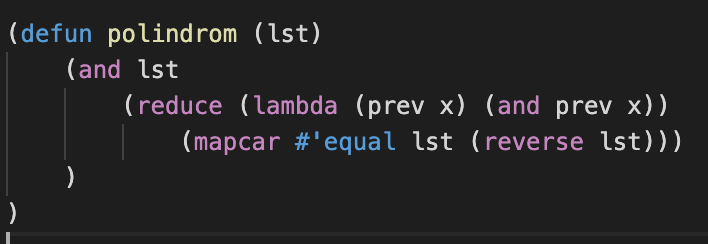
\includegraphics[scale = 1.0]{1.png}}
 			\label{ris:1}
 		\end{center}
 		\caption{Функция, проверяющая список на полиндром}
 	\end{figure}
 	
 	\subsection*{Назначение параметров функций}
 	
 	\begin{itemize}
 		\item Функционал mapcar возвращает список типа (nil t t nil nil)
 		\item Функционал reduce применяет and для списка
 	\end{itemize}
 	
 	\subsection*{Результаты работы}
 	
 	\begin{table} [h!]
 		\begin{center}
 			\begin{tabular}{|l|l|}
 				\hline
 				{\bf  Выражение} &    {\bf Результат} \\
 				\hline
 				{'(1 2 3 4 5)} & NIL\\
 				\hline
 				{'(1 2 3 2 1)} & T\\
 				\hline
 				{'(1 2 3)} & NIL\\
 				\hline
 				{'(1)} & T\\
 				\hline
 				{'()} & NIL\\
 				\hline
 				{'((1 2) 4 (1 2))} & NIL\\
 				\hline
 			\end{tabular}  
 			\label{m1}
 		\end{center}
 	\end{table}
 	
 	\newpage
	
	\section*{4. Напишите функцию swap-first-last, которая переставляет в списке-аргументе первый и последний элементы.}
	
	\subsection*{Реализация задания}
	
	\begin{figure}[h!]
		\begin{center}
			{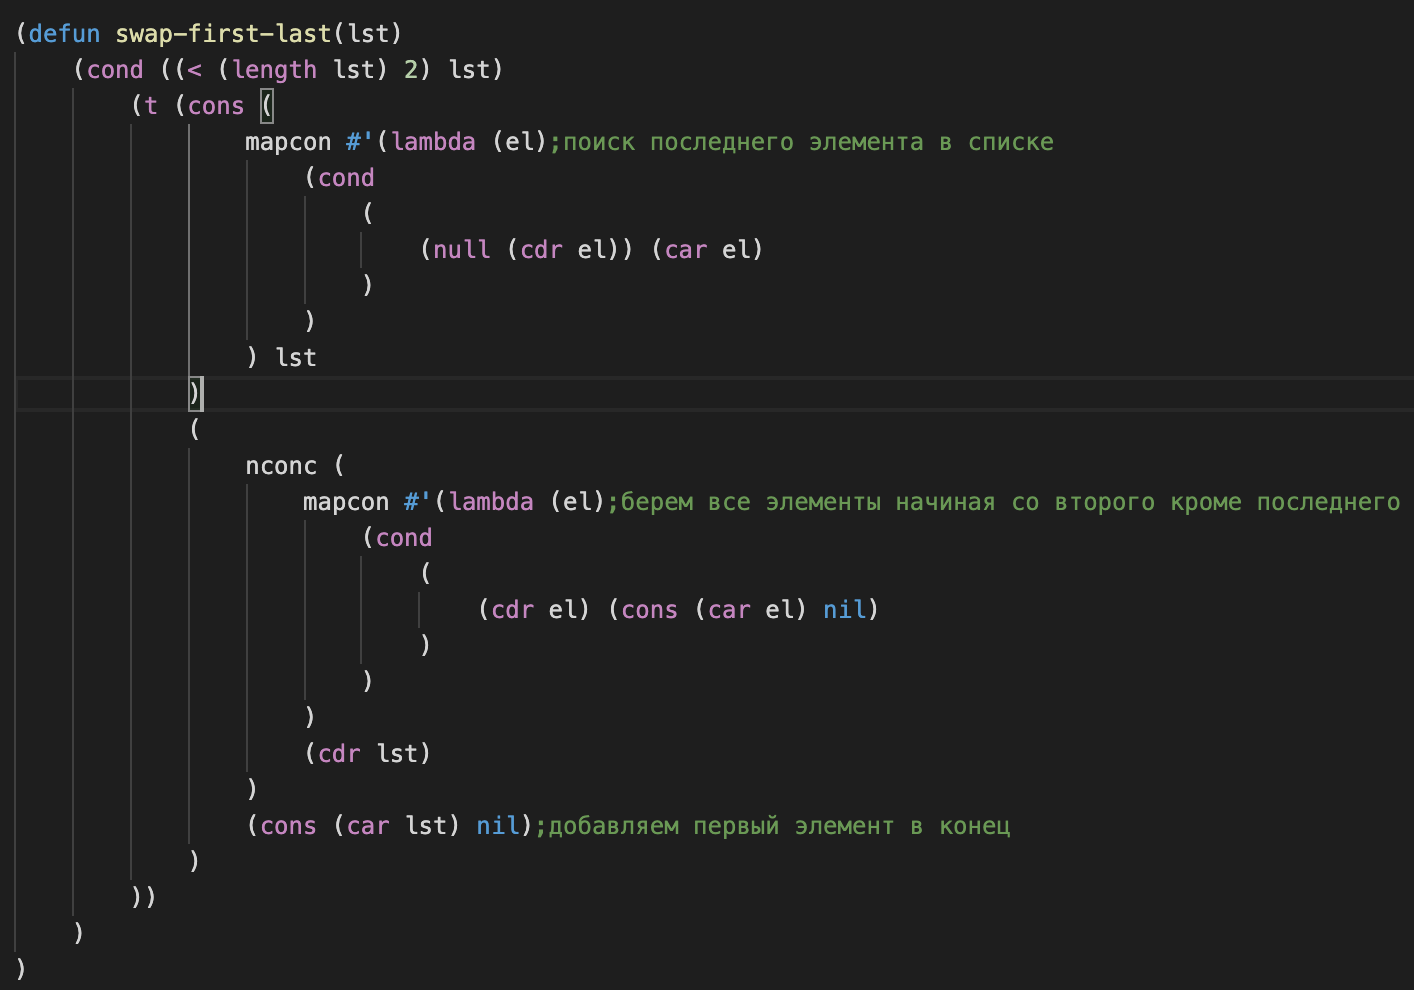
\includegraphics[scale = 0.7]{4.png}}
			\label{ris:4}
		\end{center}
		\caption{Функция, переставляющая в списке-аргументе первый и последний элементы}
	\end{figure}
	
	\subsection*{Назначение параметров функций}
	
	\begin{itemize}
		\item Первый функционал mapcon ищет последний элемент в списке
		\item Второй функционал mapcon формирует список, начиная со второго и до последнего (не включительно)
		\item Если длина списка меньше 2, то условие cond возвращает список без изменений
	\end{itemize}
	
	\subsection*{Результаты работы}
	
	\begin{table} [h!]
		\begin{center}
			\begin{tabular}{|l|l|}
				\hline
				{\bf  Выражение} &    {\bf Результат} \\
				\hline
				{'(1 2 3 4 5 6)} & (6 2 3 4 5 1)\\
				\hline
				{'(1 2 3 4 5 (1 2))} & ((1 2) 2 3 4 5 1)\\
				\hline
				{'(1 2)} & (2 1)\\
				\hline
				{'(1)} & (1)\\
				\hline
				{'()} & NIL\\
				\hline
			\end{tabular}  
			\label{m2}
		\end{center}
	\end{table}
	
	 \newpage
	
	\section*{5. Напишите функцию swap-two-element, которая переставляет в списке-аргументе два указанных своими порядковыми номерами элемента в этом списке.}
	
	\subsection*{Реализация задания}
	
	\begin{figure}[h!]
		\begin{center}
			{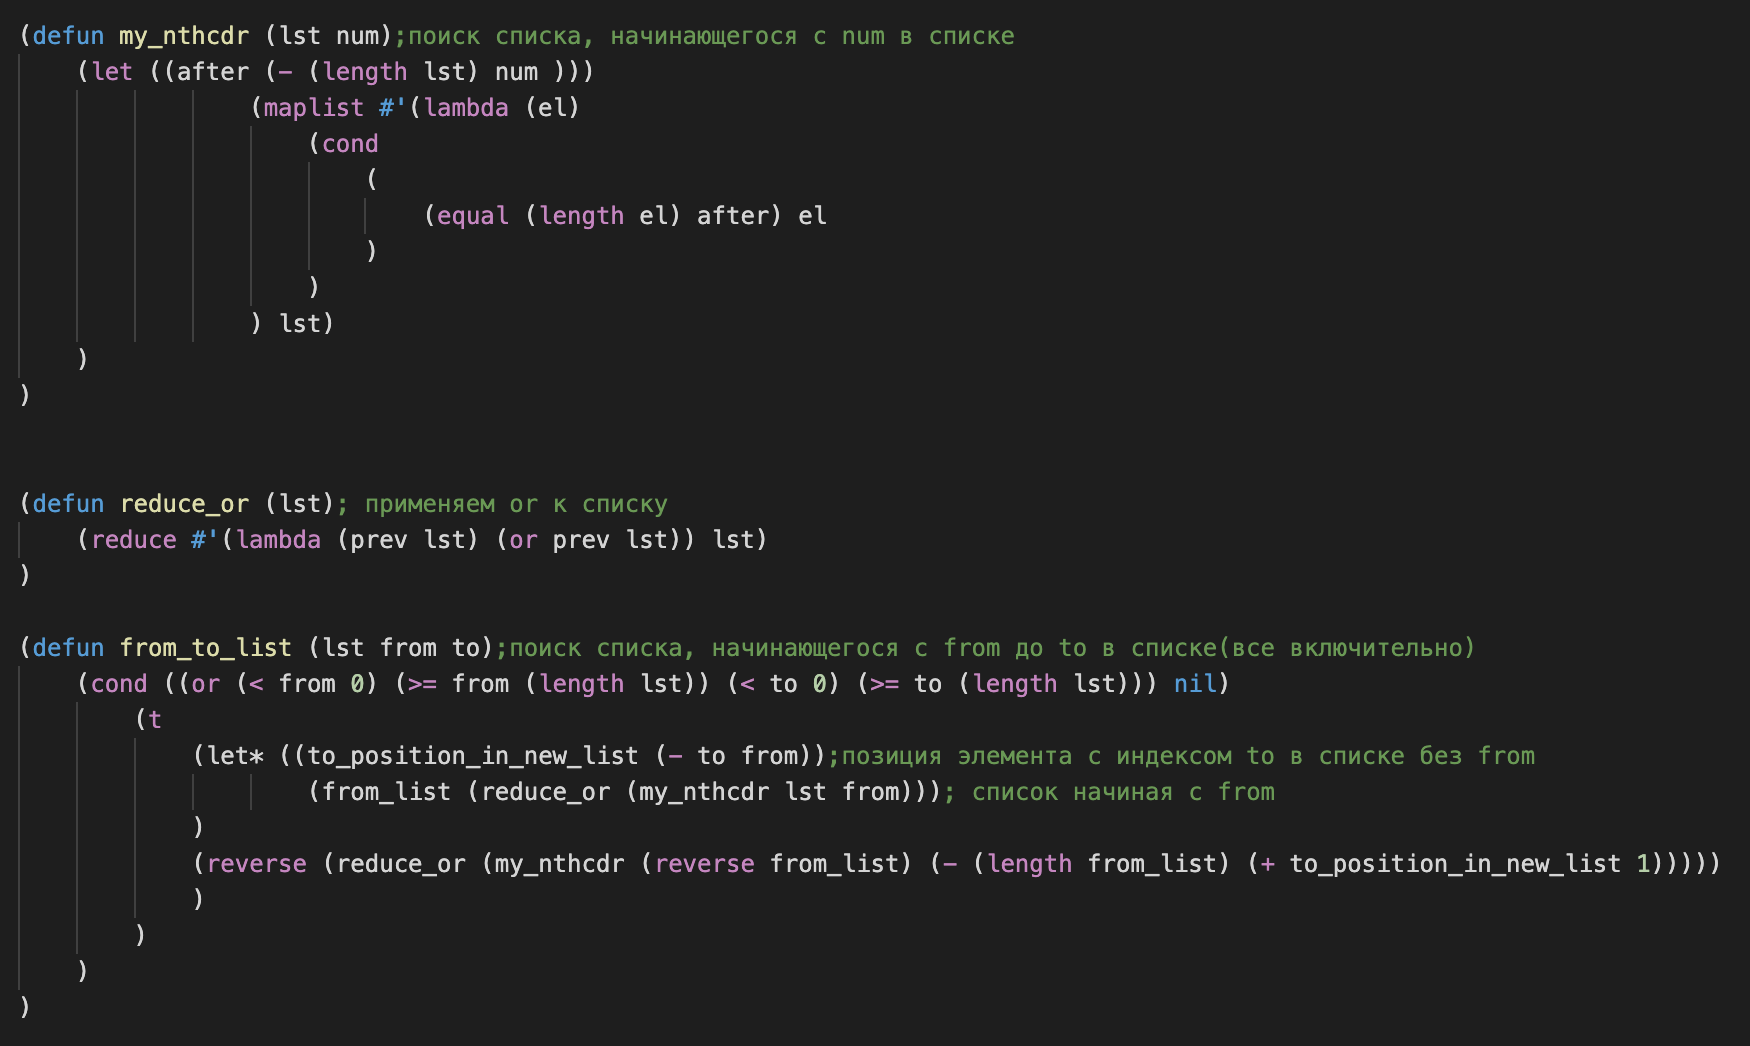
\includegraphics[scale = 0.6]{5.2.png}}
			\label{ris:5.2}
		\end{center}
	\caption{Вспомогательные функции для swap-two-element}
	\end{figure}

	\begin{figure}[h!]
		\begin{center}
			{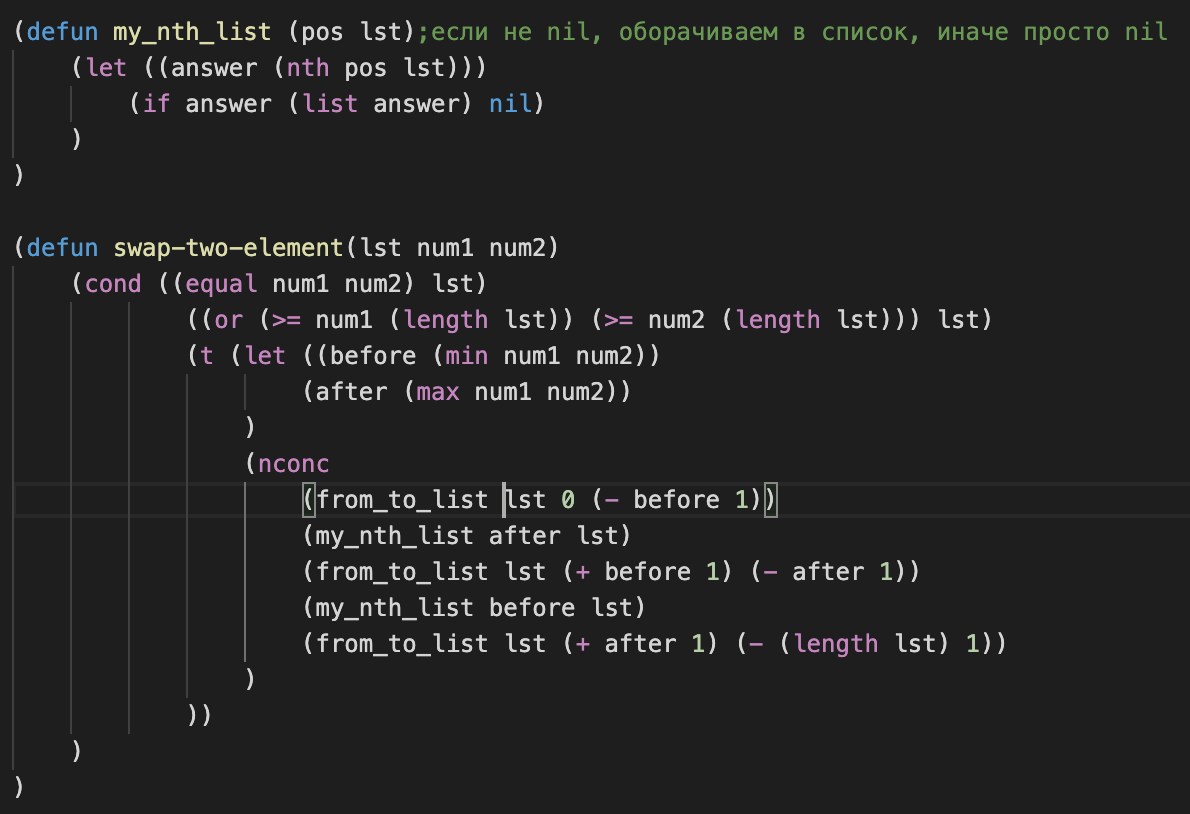
\includegraphics[scale = 0.8]{5.1.png}}
			\label{ris:5.1}
		\end{center}
	\caption{Функция, переставляющая в списке-аргументе два указанных своими порядковыми номерами эемента в этом списке}
	\end{figure}

	\newpage
	
	\subsection*{Назначение параметров функций}
	
	\begin{itemize}
		\item Параметр before - минимальное число из num1 и num2
		\item Параметр after - максимальное число из num1 и num2
		\item Далее формируем и конкатенируем следующие списки из списка lst: (от нуля и до before - 1); (after); (от before + 1 и до after - 1); (before); (от after + 1 и до конца списка)
		\item Функция my\_nth\_list возвращает элемент из списка на позиции pos, оборачивая его в список, если он не nil
		\item Фцункция from\_to\_list формирует список из списка-параметра, начиная с позиции from и до to (включительно)
		\item Функция reduce\_or применяет or к списку
		\item Функция my\_nthcdr возвращает хвост списка lst, начиная с позиции num
	\end{itemize}
	
	\newpage
	
	\subsection*{Результаты работы}
	
	\begin{table} [h!]
		\begin{center}
			\begin{tabular}{|l|l|}
				\hline
				{\bf  Выражение} &    {\bf Результат} \\
				\hline
				{'(1 2 3 4 5 6 7 8) 1 4} & (1 5 3 4 2 6 7 8)\\
				\hline
				{'(1 2 3 4 5 6 7 8) 4 1} & (1 5 3 4 2 6 7 8)\\
				\hline
				{'(1 2 3 4 5 6 7 8) 0 7} & (8 2 3 4 5 6 7 1)\\
				\hline
				{'(1 2 3 4 5 6 7 8) 1 8} & (1 2 3 4 5 6 7 8)\\
				\hline
				{'(1 2 3 4 5 6 7 8) 1 10} & (1 2 3 4 5 6 7 8)\\
				\hline
				{'(1 2 3 4 5 6 7 8) 1 1} & (1 2 3 4 5 6 7 8)\\
				\hline
				{'(1 2) 1 1} & (1 2)\\
				\hline
				{'(1 2) 0 1} & (2 1)\\
				\hline
				{'(1) 0 0} & (1)\\
				\hline
				{'() 0 0} & NIL\\
				\hline
			\end{tabular}  
			\label{m3}
		\end{center}
	\end{table}
	
	\newpage
	
	\section*{6. Напишите две функции, swap-to-left и swap-to-right, которые производят круговую перестановку (на k позиций) в списке-аргументе влево и вправо, соответственно.}
	
	\subsection*{Реализация задания}
	
	\begin{figure}[h!]
		\begin{center}
			{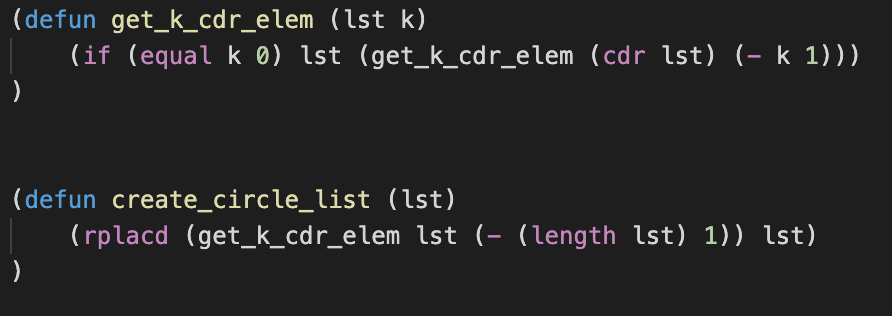
\includegraphics[scale = 0.9]{6.2.png}}
			\label{ris:6.2}
		\end{center}
	\caption{Вспомогательные функции к фукциям swap-to-left и swap-to-right}
	\end{figure}

	\begin{figure}[h!]
		\begin{center}
			{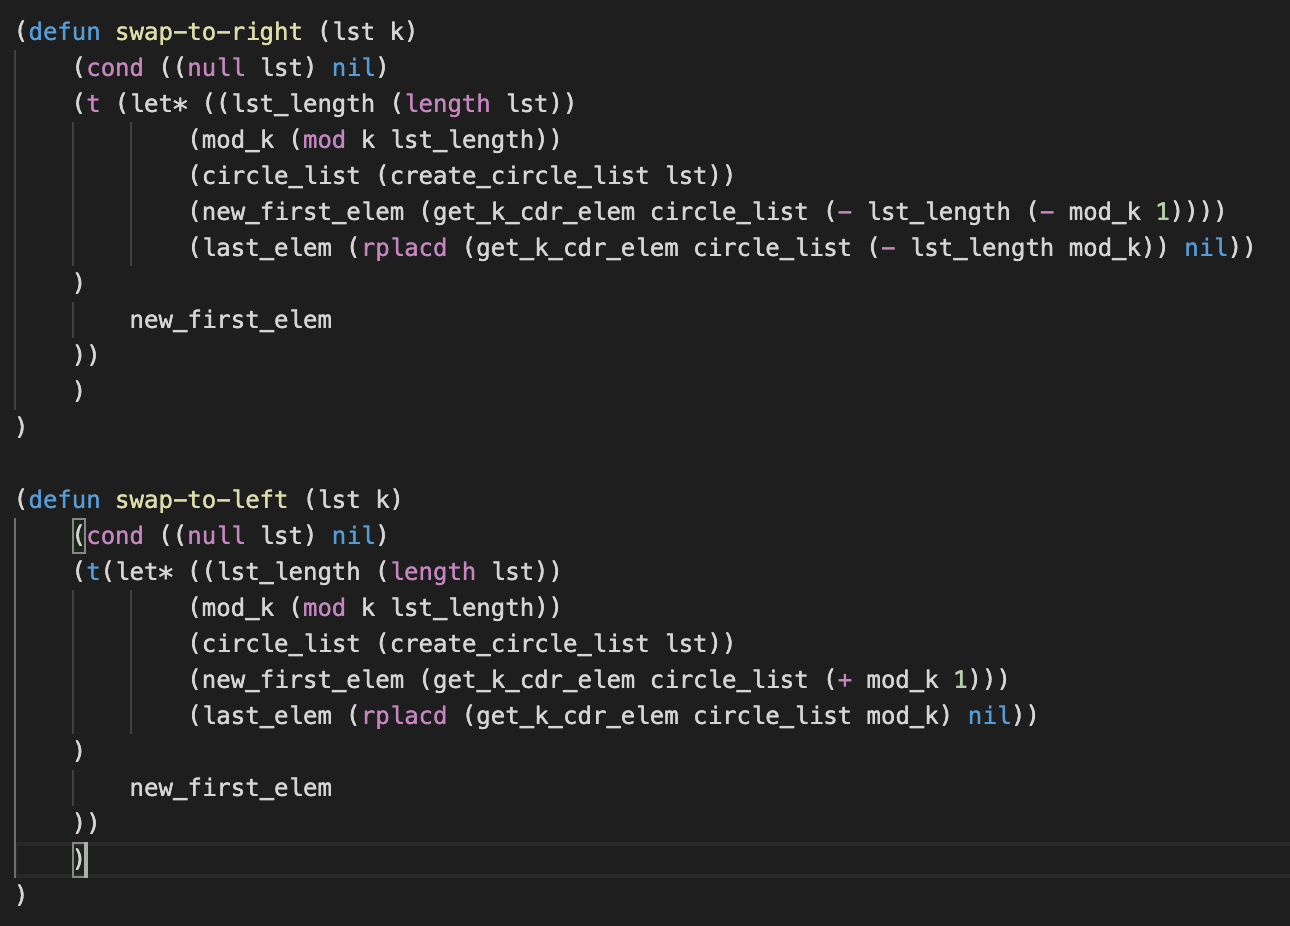
\includegraphics[scale = 0.8]{6.1.png}}
			\label{ris:6.1}
		\end{center}
	\caption{Функции, производящие круговую перестановку на k позиций в списке-аргументе влево и вправо, соответственно}
	\end{figure}

	\newpage
	
	\subsection*{Назначение параметров функций}
	
	\begin{itemize}
		\item Переменная lst\_length обозначает длину первоначального списка (до его изменения функцией rplacd)
		\item Переменная mod\_k берет остаток от деления k на длину списка
		\item Переменная new\_first\_elem - новая голова списка
		\item Переменная last\_elem - результат работы функции get\_k\_cdr\_elem (последний элемент списка)
		\item Функция create\_circle\_list делает список lst кольцевым (переставляет указатель последнего элемента на голову списка и возвращает этот последний элемент)
		\item Функция get\_k\_cdr\_elem идет по списку и возвращает указатель на его элемент через k позиций
		\item Функция swap\_to\_right аналогична функции swap\_to\_left за исключением того, что она сдвигает список на length(lst) - (k + 1) позиций вместо (k + 1)
	\end{itemize}
	
	\subsection*{Результаты работы}
	
	\begin{table} [h!]
		\begin{center}
			\begin{tabular}{|l|l|l|}
				\hline
				{\bf  Выражение} &  {\bf Результат swap\_to\_left} &  {\bf Результат swap\_to\_right}\\
				\hline
				{'(1 2 3 4 5 6) 3} & (4 5 6 1 2 3) & (4 5 6 1 2 3)\\
				\hline
				{'(1 2 3 4 5 6) 6} & (1 2 3 4 5 6) & (1 2 3 4 5 6)\\
				\hline
				{'(1 2 3 4 5 6) 9} & (4 5 6 1 2 3) & (4 5 6 1 2 3)\\
				\hline
				{'(1 2 3 4 5 6) 0} & (1 2 3 4 5 6) & (1 2 3 4 5 6)\\
				\hline
				{'(1 2 3 4 5 6) 2} & (3 4 5 6 1 2) & (5 6 1 2 3 4)\\
				\hline
				{'(1) 0} & (1) & (1)\\
				\hline
				{'(1) 3} & (1) & (1)\\
				\hline
				{'(1) 0} & (1) & (1)\\
				\hline
				{'() 0} & NIL & NIL\\
				\hline
			\end{tabular}  
			\label{m4}
		\end{center}
	\end{table}
	
	\newpage
	
	\section*{7. Напишите функцию, которая умножает на заданное число-аргумент все числа
из заданного списка-аргумента, когда
a) все элементы списка --- числа,
б) элементы списка -- любые объекты.
	}
	
	\subsection*{Реализация задания}
	
	\begin{figure}[h!]
		\begin{center}
			{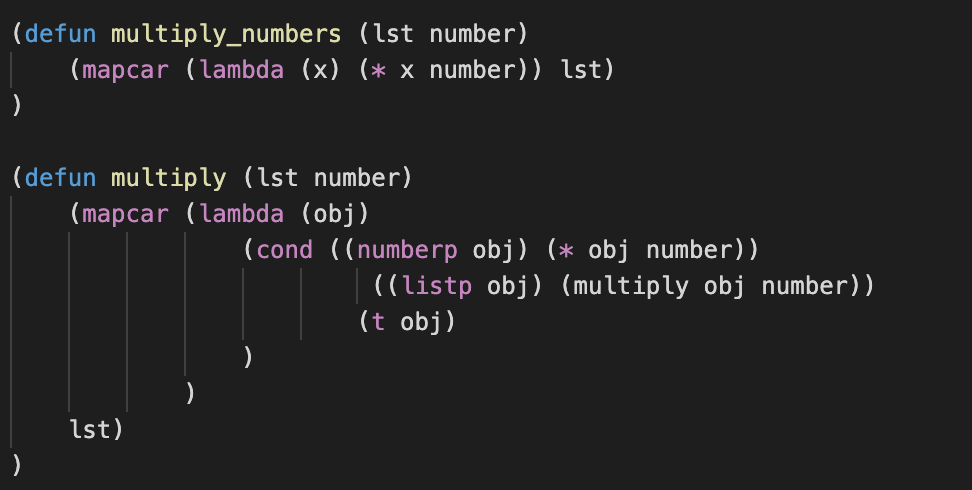
\includegraphics[scale = 1.0]{7.png}}
			\label{ris:7}
		\end{center}
	\caption{Функции multiply\_numbers (элементы списка - числа) и multiply (элементы списка - любые объекты), умножающие число-аргумент на числа списка-аргумента}
	\end{figure}
	
	\subsection*{Назначение параметров функций}
	
	\begin{itemize}
		\item Функция multiply\_numbers выполняет пункт а из задания
		\item Функция multiply выполняет пункт б из задания, используя проверку на число (функция numberp) и проверку на список (функция listp)
	\end{itemize}
	
	\subsection*{Результаты работы}
	
	\begin{table} [h!]
		\begin{center}
			\begin{tabular}{|l|l|l|}
				\hline
				{\bf  Выражение} & {\bf Результат multiply\_numbers} & {\bf Результат multiply} \\
				\hline
				{'(1 2 3 4 5 6) 3} & (3 6 9 12 15 18) & (3 6 9 12 15 18)\\
				\hline
				{'(1 2 3 4 5 6) 0} & (0 0 0 0 0 0) & (0 0 0 0 0 0)\\
				\hline
				{'(1 2 3 4 5 6) 1} & (1 2 3 4 5 6) & (1 2 3 4 5 6)\\
				\hline
				{'() 5} & NIL & NIL\\
				\hline
				{'(1 2 3 (1 2) 4 5) 4} & --- & (4 8 12 (4 8) 16 20)\\
				\hline 
				{'(1 2 3 (1 2 (a 3)) 4 5) 6} & --- & (6 12 18 (6 12 (A 18)) 24 30)\\
			\end{tabular}  
			\label{m5}
		\end{center}
	\end{table}
	
	
	\newpage
	
	\section*{8. Напишите функцию, select-between, которая из списка-аргумента,
содержащего только числа, выбирает только те, которые расположены между двумя указанными границами-аргументами и возвращает их в виде списка (упорядоченного по возрастанию списка чисел (+ 2 балла)).
	}
	
	\subsection*{Реализация задания}
	
	\begin{figure}[h!]
		\begin{center}
			{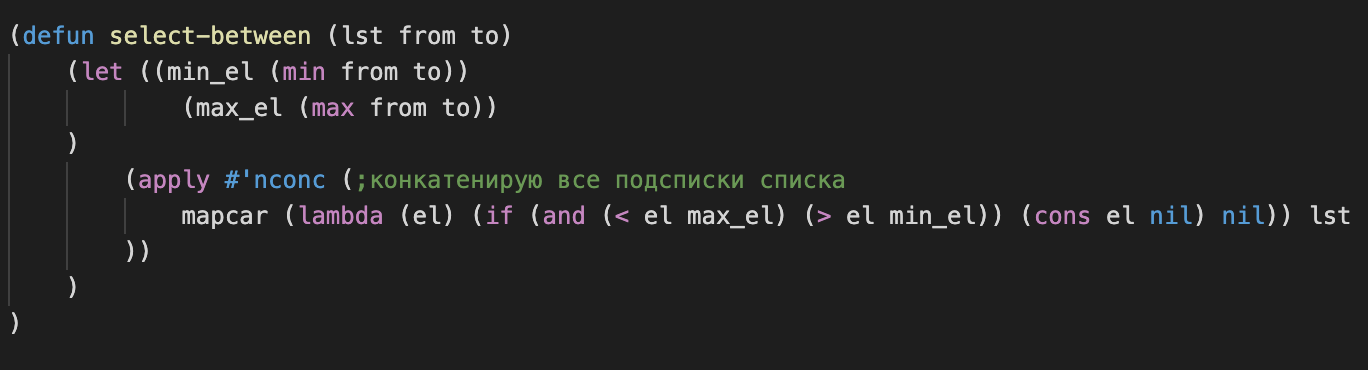
\includegraphics[scale = 0.7]{8.1.png}}
			\label{ris:8.1}
		\end{center}
	\caption{Функция, выбирающая из списка-аргумента элементы меньшие to и большие from}
	\end{figure}

	\begin{figure}[h!]
		\begin{center}
			{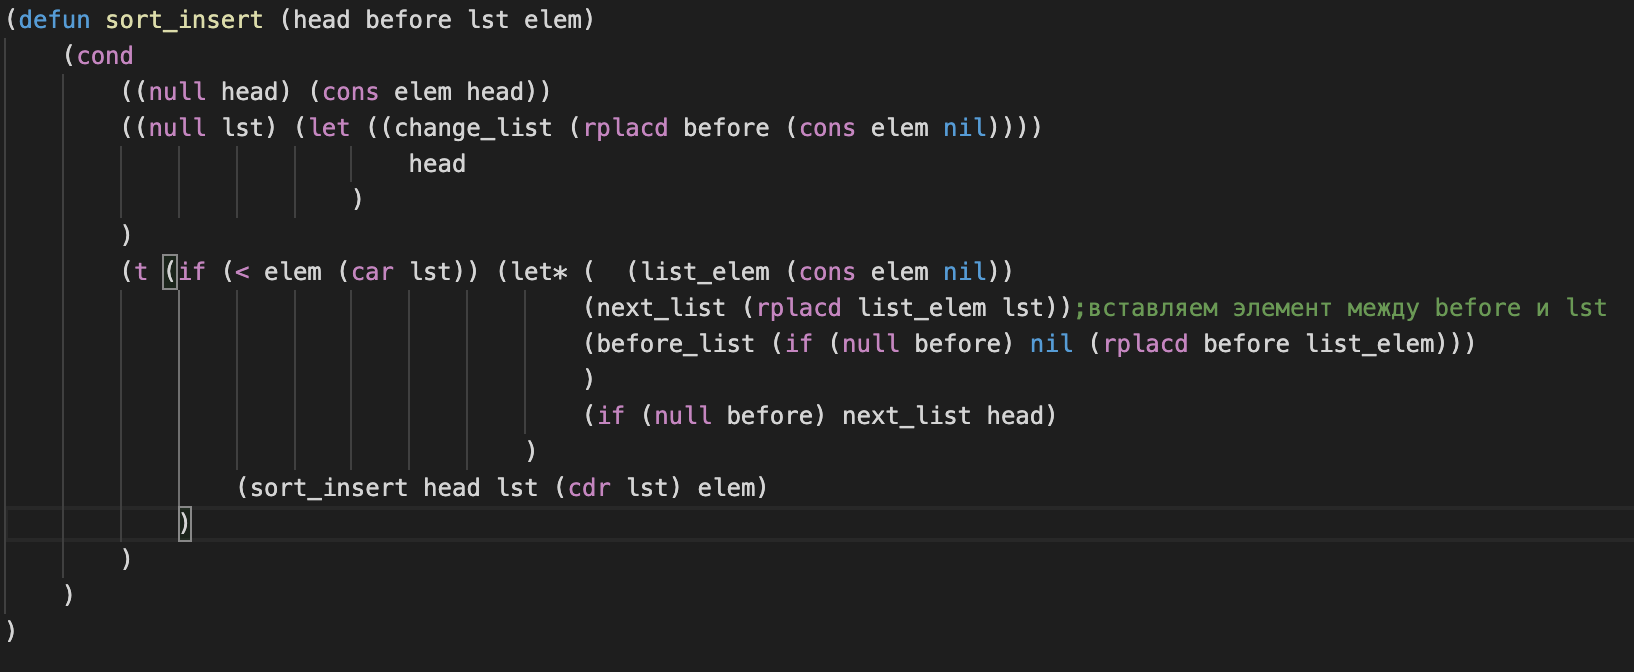
\includegraphics[scale = 0.65]{8.3.png}}
			\label{ris:8.2}
		\end{center}
	\caption{Вспомогательная функция сортировки для функции select-between}
	\end{figure}

	\newpage

	\begin{figure}[h!]
		\begin{center}
			{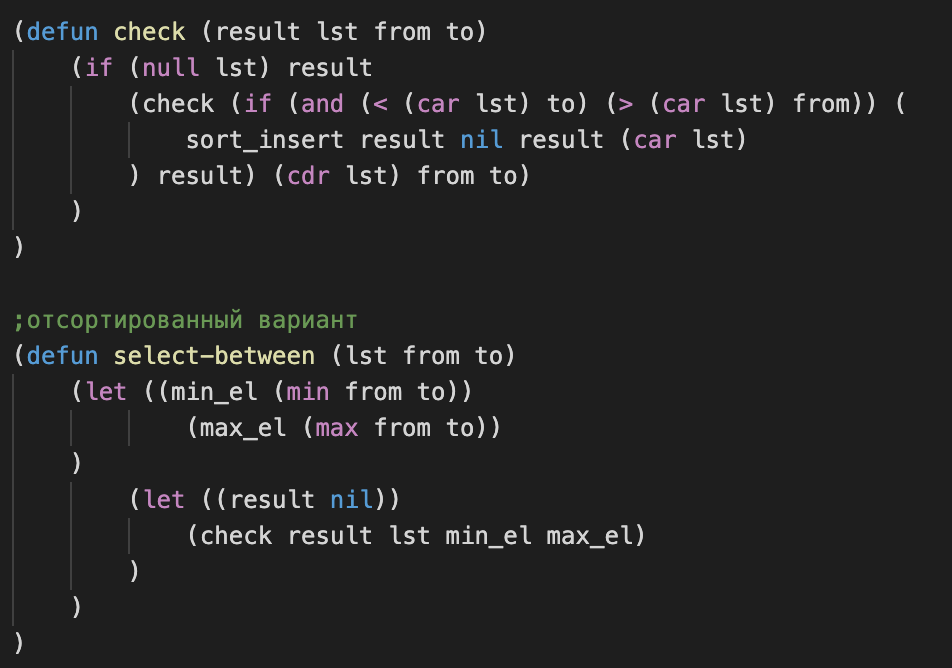
\includegraphics[scale = 1.0]{8.2.png}}
			\label{ris:8.3}
		\end{center}
	\caption{Функция, выбирающая из списка-аргумента элементы меньшие to и большие from и сортирующая их по возрастанию}
	\end{figure}
	
	\subsection*{Назначение параметров функций}
	
	\begin{itemize}
		\item Переменные min\_el, max\_el - минимальные и максимальные границы из from и to соответственно
		\item Идея фнкции sort\_insert аналогична сортировке вставками: вставляет число-аргумент перед ближайшим большим элементом списка-аргумента в этот список
		\item Переменная head - голова списка
		\item Переменная before - предыдущий элемент списка (изначально nil)
		\item Переменная change\_list - результат работы функции rplacd, которая перебрасывает указатель элемента списка before на elem
		\item Переменная next\_list - результат работы функции rplacd, вставляющей elem в голову списка lst
		\item Переменная before\_list - результат работы функции rplacd, которая перебрасывает указатель элемента списка before на elem, если before не null
		\item Функция check - хвостовая рекурсивная функция, аналогичная select-between без сортировки
	\end{itemize}
	
	\subsection*{Результаты работы}
	
	\begin{table} [h!]
		\begin{center}
			\begin{tabular}{|l|l|l|}
				\hline
				{\bf  Выражение} & {\bf Результат select-between} & {\bf Результат сорт. select-between}  \\
				\hline
				{'(1 9 7 3 4 6 8 2 5) 3 7} & (4 6 5) & (4 5 6)\\
				\hline
				{'(1 9 7 3 4 6 8 2 5) 0 10} & (1 9 7 3 4 6 8 2 5) & (1 2 3 4 5 6 7 8 9)\\
				\hline
				{'(1 9 7 3 4 6 8 2 5) 7 3} & (4 6 5) & (4 5 6)\\
				\hline
				{'(1 9 7 3 4 6 8 2 5) 3 3} & NIL & NIL\\
				\hline
				{'(1 9 7 3 4 6 8 2 5) 3.3 4.3} & (4) & (4)\\
				\hline
				{'(1 9) 3.3 4.3} & NIL & NIL \\
				\hline
				{'(1 9) 10.3 9.3} & NIL & NIL \\
				\hline
				{'(1) 0.3 1.3} & (1) & (1) \\
				\hline
				{'()  0.3 1.3} & NIL & NIL \\
				\hline
			\end{tabular}  
			\label{m6}
		\end{center}
	\end{table}
	

\end{document}